\chapter{Machine Learning for Speech}\label{ch:machine_learning}

\section{Historical Overview}
Markov Model, ETC...\\\\
Rise of Artificial Neural Network...\\\\
This brain modeling approach is a less technical way to develop machine learning solutions, but it is known to be more efficient and accurate than previous traditional approaches,
such as the Hidden Markov Model (HMM). 

\subsubsection{Hidden Markov Model}
HMM takes it`s name from the fact that the state of the machine is always hidden from the user. 
The forward and backward recursions used in HMM  were created by Ruslan L. Stratonovich in 1960 \cite{stratonovich1960conditional}.
HMM takes it`s name from the fact that the state of the machine is always hidden from the user. One of the first applications of HMMs was speech recognition, starting in the mid-1970s.


\section{Artificial Neural Networks}
%---------------------------------------------------
\subsection{What is an Artificial Neural Network?}
Artificial Neural Networks are nothing but a computerized representation of the human brain. 
They have the ability to acquire and maintain knowledge (information based) and can be defined as a set of processing units, represented by artificial neurons,
interlinked by a lot of interconnections
(artificial synapses) \cite[p.~5]{Silva2016}.\\\\
The human brain learns from its experiences, creating new neural pathways. These interconnected chains of neurons are stronger than others and can be modulated, or changed,
following learning or during behavioural modifications.
The strongness of a neural connection is given by a weighted value, called synaptic weights.

\subsection{Artificial Neuron}
The Artificial neuron is the processing unit of an artificial neural network, which is a simplified model of the biological neuron.
This model was inspired by the analysis of how a cell membrane of a neuron generates and propagates electrical impulses(Hodgkin and Huxley 1952) \cite[p.~11]{Silva2016}.
The purpose of artificial neurons is to simulate the basic function of biological ones,
which are typically comprised of four parts:

\begin{enumerate}
	\item Dendrites: Accept inputs
	\item Soma(Cell body): Process the inputs
	\item Axon: Turn the processed inputs into outputs
	\item Synapses: The electrochemical connections between neurons 
\end{enumerate}
The following figure illustrates the four main functions of a biological neuron, represented on the artificial one. 

The artificial neurons used in artificial neural networks are non-linear, usually providing continuous outputs,
and performing simple functions,
such as gathering signals available on their inputs,
assembling them according to their operational functions,
and producing a response considering their innate activation functions \cite[p.~11]{Silva2016}. 

\begin{figure}[h]
\centering
	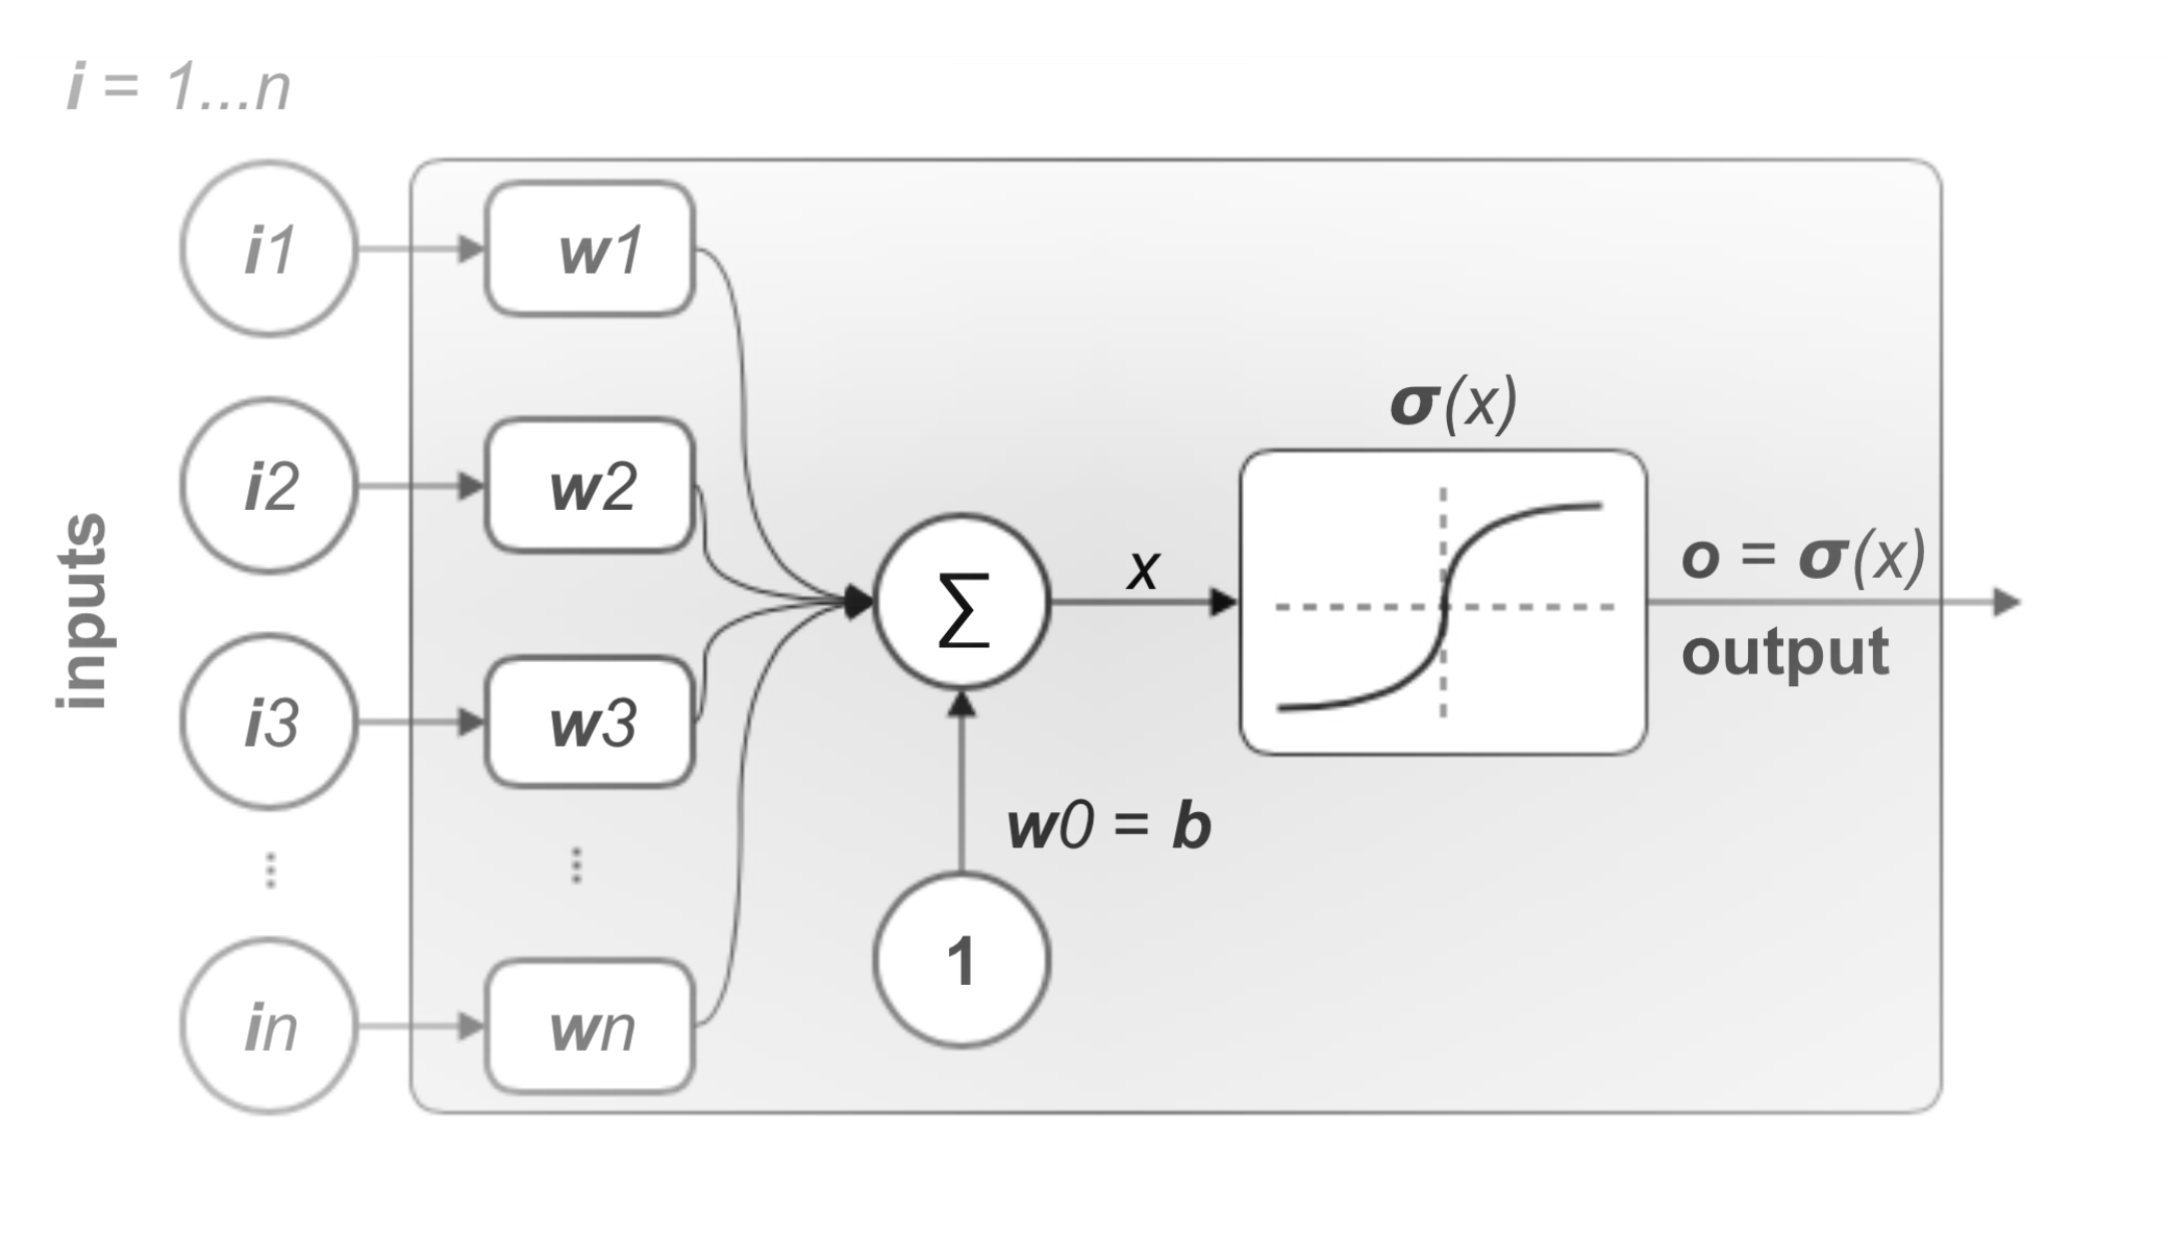
\includegraphics[width=\textwidth]
	{machine_learning/00_Artificial_Neuron}
	\caption{The artificial neuron.}
	\label{fig:AN}
\end{figure}

Each neuron from a network can be implemented as shown in Fig.
\ref{fig:AN}. The multiple input signals coming from the external environment are represented by the set
$\left\{i1,i2,i3,...,in \right\}$, analogous to the external electrical impulses gathered by the dendrites in the biological neuron.
\todo{re-write}

%---------------------------------------------------

\section{Types of Artificial Neural Networks}
%---------------------------------------------------
 
\subsection{Feed forward Network}


This type of simple neural network is comprised of one input
layer and one neural layer, which also acts as the output layer.
The flow of information is uni directional, starting from the input layer and progressing to the output layer. As such, the number of outputs from the neural network will always coincide with the number of neurons in the network.
 These networks are usually employed in
pattern classification and linear filtering problems. 
The Perceptron and the ADALINE architectures are among the most recognised feed-forward neural networks and they work well with Hebb`s rule and the Delta rule for training.

\subsection{Deep Recurrent Neural Network}
To explain how a deep recurrent neural network(RNN) looks like first we will see what a deep neural network is made of and after that the recurrent part will be added to form a more complex and and powerful network.

Networks with multiple layers are have one or more hidden neural layers. Such a network will always have one input layer with multiple samples and a series of variable layers.
In contrast to the simple feed-forward network, these hidden layers are not constrained to have the same size as the input layer. This means
that the size can depend on the complexity of the problem being
tackled by the network, as well as the quantity and quality of the available data. The last layer still occupies a double role as both a neuron layer and output layer.

Another key element is the fact that the outputs of the neurons  are used for feedback inputs to the other neurons.
This feature makes the network great for time-variant systems where the new outputs can benefit from previous information.

\subsection{Long Short Term Memory}
Long Short Term Memory networks, for short “LSTMs”, are a special case of recurrent neural network that  capable of learning long-term dependencies.
Firstly used in 1997 by Sepp Hochreiter and Jürgen Schmidhuber \cite{Father} and refined by Felix Gers and his team \cite{Gers99}.
Nowadays, after further refinement,
LSTMs work incredibly well on various problems and give better results for most problems that require RNNs.
They remember information for long periods of time by default, making them the perfect fit to avoid long-term dependency problems. 

LSTMs have a chain like structure of four layers, with repeating modules that interact in  specific ways. For simplicity, in the following explanation of the internal states of a LSTM, the input X will represent the normal input to the network concatenated with the previous state, $X = x_i | h_{t-1}$.

\begin{figure}[H]
	\centering
	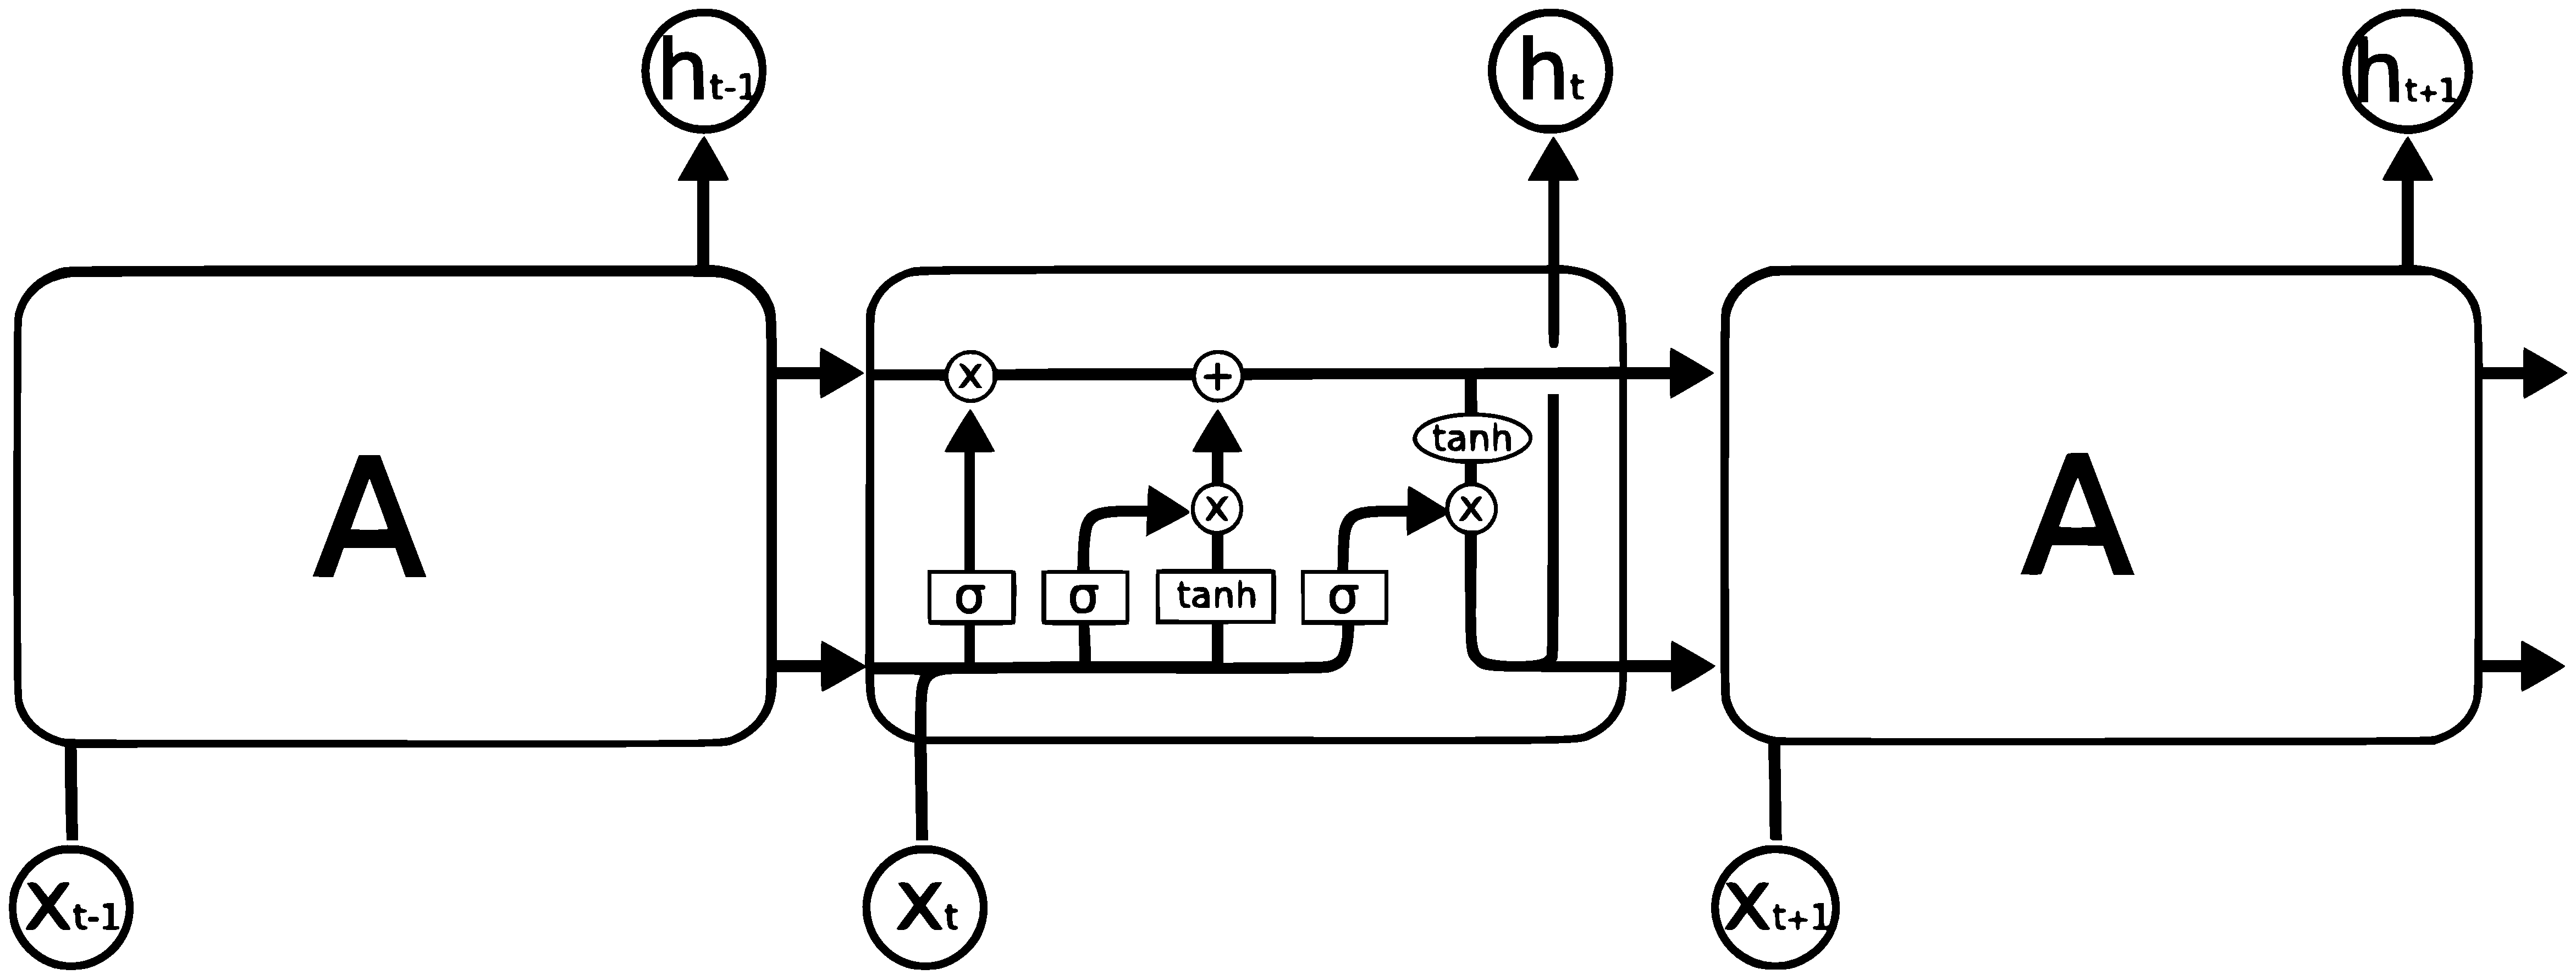
\includegraphics[width=\textwidth]	
	{machine_learning/01_Lstm_Diagram}
	\caption{LSTM Diagram.}
	\label{fig:LSTM1}
\end{figure}

\begin{figure}[H]
	\centering
	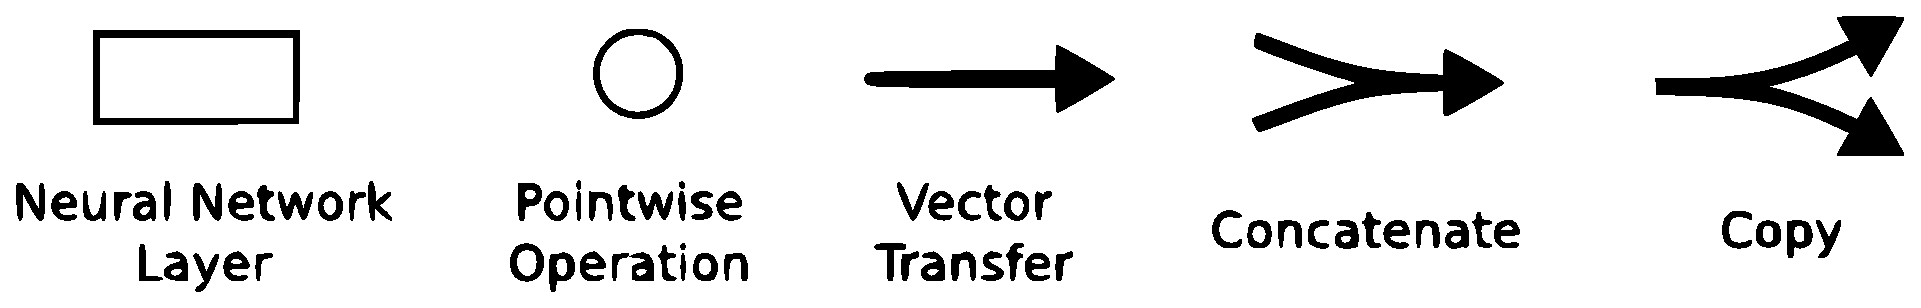
\includegraphics[width=\textwidth]		
	{machine_learning/02_Lstm_Notation}
	\caption{Diagram legend.}
	\label{fig:LSTM2}
\end{figure}

From the legend above, the lines represent
vectors that pass from the output of the
previous note to the input of the current one.
The dot denotes point wise operations, 
and the rectangle represents trained network
layers.


A side by side description of the each layer of a LSTM and it`s mathematical formulation can be seen below, where the dot represents matrix multiplication.
The first layer represents the forget gate. This is where we decide which information to keep and which to discard. The layer outputs a value between zero and one for each input because of the sigmoid function(represented as sigma in the equations below), meaning that a value of zero represents data that will be complicity erased and so forth, while an absolute value of one represents data that will be left unchanged for the next iteration.    

\begin{figure}[H]
	\centering
	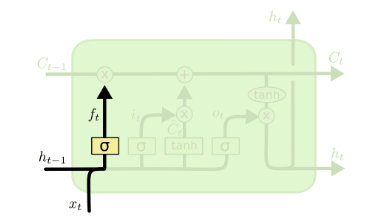
\includegraphics[width=0.5\textwidth]		
	{machine_learning/03_RForget}
	\begin{equation}
		 f= \sigma*(X.W_f+b_f) 
	\end{equation}	
	\caption{Forget Gate for concatenated inputs.}
	\label{fig:Forget}
\end{figure}

Similar to the forget gate, the LSTM structure also uses an update gate, to add new information to the system.
As seen in Figure \ref{fig:Update}, the update gate generates the new values that will be used. This takes place by multiplying the update gate to the input layer, represented by X` where a  hyperbolic tangent is used as the activation function. This is given as an example, as the Rectified Linear Unit(ReLU) or the softmax activation work perfectly fine as well.  
From the above mentioned gates a new internal state C can be computed as:
\begin{equation}
C_t= f * C_{t-1} + u*X` 
\end{equation}
Where the current state ($C_t$) is determined by what we want to forget ($f$), multiplied by the previous state ($C_t-1$) and added together with the update gate ($r$) times the input layer ($X`$).

\begin{figure}[H]
	\centering
	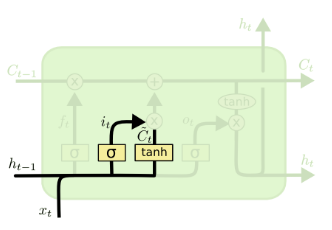
\includegraphics[width=0.5\textwidth]		
	{machine_learning/04_Update}
	\begin{equation}
		 f= \sigma*(X.W_u+b_u) 
	\end{equation}	
	\begin{equation}	 
		 X`=tanh*(X.W_c+b_c)
	 \end{equation}
	\caption{Update gate with the current state description.}
	\label{fig:Update}
\end{figure}

\begin{figure}[H]
	\centering
	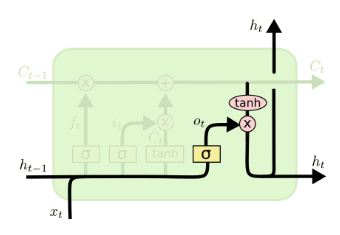
\includegraphics[width=0.5\textwidth]		
	{machine_learning/05_Result}
	\begin{equation}
		 r= \sigma*(X.W_r+b_r) 
	\end{equation}	
	\caption{Result gate added to the output function.}
	\label{fig:Result}
\end{figure}

The third and last gate is the result gate ($r$), which uses the previous internal state of the LSTM to generate a new internal state.
As such, the output of the neural network can be written as:

\begin{equation}
Y_t=softmax(H_t.W+b)
\end{equation}
%---------------------------------------------------
\subsection{Dropout}
Dropout is a regularization technique that involves shooting the neurons.
It is applied after the activation function of each layer with the notable exception of the input and output layer.
A percentage is used to determine the number of neurons that will remain in the networks.
For example, a .75 value in the dropout function means that only 75 percent of the neurons will remain active during the training phase.
At the test time all the neurons have to be present, meaning that a value of 1 has to be given to the dropout function to ensure a high accuracy rating.
This helps the network understand the information it is given as it cannot presume that other neurons in the same layer have been activated and it prevents the network from just memorizing the values that were given as inputs.
The snipped below shows how dropout is used in TensorFlow for a layer of a neural network, where pkeep is the percentage of the neurons that will remain active and the call for the dropout is made after the activation function, in this case the ReLU.
\begin{lstlisting}
pkeep = tf.palceholder(tf.float32)
YF = tf.nn.relu(tf.matmul(X, W)+ b)
Y = tf.nn.dropout(Yf, pkeep)
\end{lstlisting} 

\begin{figure}[H]
	\centering
	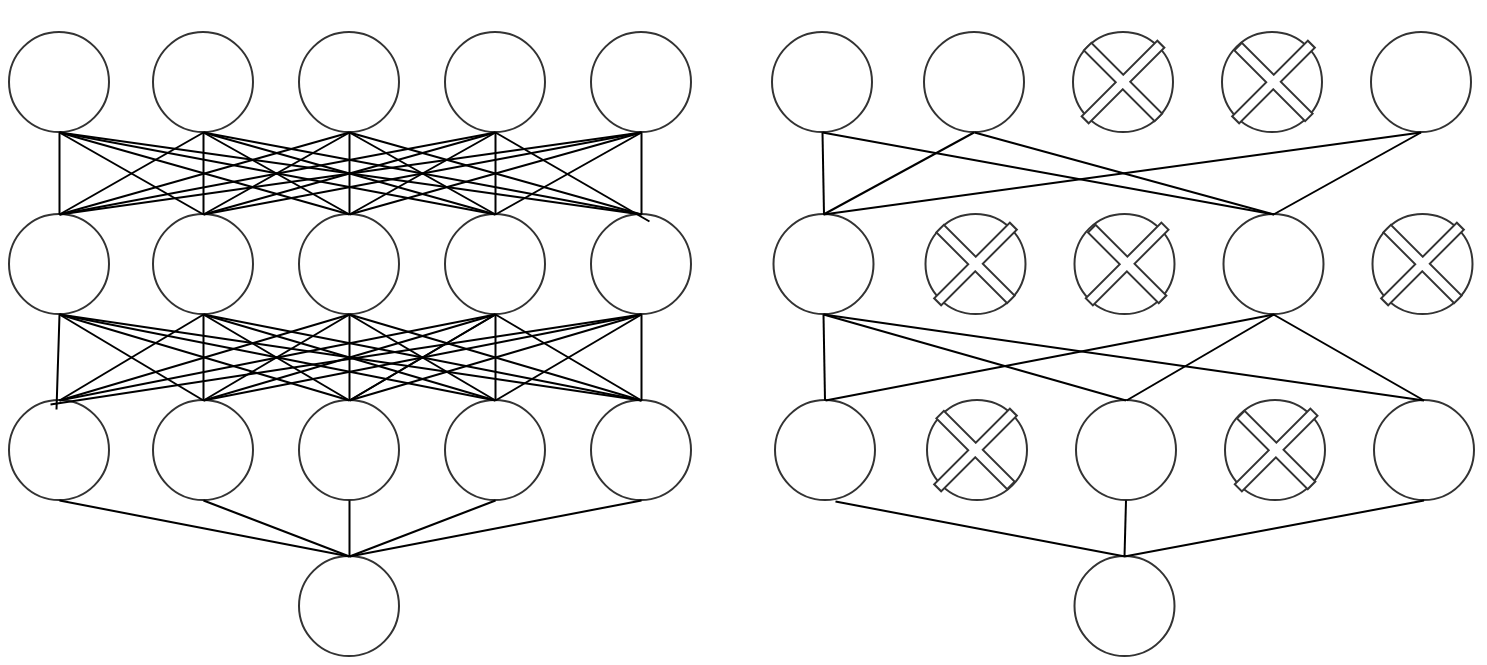
\includegraphics[width=\textwidth]		
	{machine_learning/06_Dropout}

	\caption{Dropout used on a generic network.}
	\label{fig:Result}
\end{figure}


%---------------------------------------------------
\subsection{Batch normalisation}

Statistics can be computed for each batch that is fed to the neural network so the average and the standard deviation can be computed. After computing them, subtracting the average and dividing by the standard deviation rescales and recentre the output. 
In the equation, epsilon is added to avoid numerical problems as dividing by zero.
\begin{equation}
X= \dfrac{x - avg(x)}{stdev(x) + \epsilon} 
\end{equation}

The recentre and rescaling of the values can cause problems to the network for cases where data needs to be squeezed over to one side of the spectrum.
To solve those cases, two degrees of freedom are added, $\alpha$ and $\beta$, for each neuron. 
By assigning the $\alpha$ value to the $stdev(x)$ and the $\beta$ to $-avg(x)$ there will always be a case where the batch normalised value of x can be reverted to the original value.
\begin{equation}
BN(x) = \alpha * X + \beta
\end{equation}
Batch normalisation(BN) is added before the activation function because it takes use of the current weights and biases to compute the average and standard deviation. 
The average and standard deviation is always computed on the current weights and biases so the batch normalisation layer is called between the weighted sum performed by the neurons and the activation function.
Because of the new values added by BN, biases are no longer useful.
The $\beta$ value can take the value of the bias if no better value was found.
In contrast to the ReLU, when using a sigmoid, the scale parameter has to be used to make sure that the data fits in the useful part of the activation function. A representation of how to choose the right coefficients is given in Table \ref{tab:Parameters}.


\begin{table}[htbp]
\centering
\begin{tabular}{lcc}
\toprule
  & ReLU & Sigmoid \\\midrule
Without BN &b & b  \\
With BN & $\beta$ & $\alpha$, $\beta$  \\
\bottomrule
\end{tabular}
\caption{Parameters for different activation functions.}
\label{tab:Parameters}
\end{table}

%---------------------------------------------------
\section{TensorFlow}

%---------------------------------------------------
TensorFlow provides multiple Application Programming Interfaces
(APIs) for machine learning. 
The lowest level API "TensorFlow Core" provides complete programming control \cite{tensorflow2015-whitepaper}. 
For those who require fine levels of control over their models,
TensorFlow Core is a well-suited tool for the job. There are higher level APIs that are built on top of TensorFlow Core.
These higher level APIs are typically easier to learn and use than Tensorflow Core \cite{tensorflow2015-whitepaper}.
In addition, the higher level APIs such as "tf.estimator" helps with managing data sets, estimators,
training and inferences (testing your trained network),
as well as, making repetitive tasks easier and more consistent
\cite{tensorflow2015-whitepaper}.\\

The subsection below will start with TensorFlow Core. 
In order to gain an understanding of the basic principles that TensorFlow has to offer, a model shall be made. 
In the subsection after that, the same model will be implemented with tf.estimator. 
Knowing TensorFlow Core principles will give us a great mental model of how things are working internally when we use the more compact higher level API.

\subsection{Tensors}
The central unit of data in TensorFlow is the tensor. 
A tensor consists of a set of primitive values shaped into an array of any number of dimensions. 
A tensor's rank is its number of dimensions. 
Here are some examples of tensors:

\begin{adjustbox}{width=\textwidth}
\begin{lstlisting}
3 # a rank 0 tensor; this is a scalar with shape []
[1., 2., 3.] # a rank 1 tensor; this is a vector with shape [3]
[[1., 2., 3.], [4., 5., 6.]] # a rank 2 tensor; a matrix with shape [2, 3]
[[[1., 2., 3.]], [[7., 8., 9.]]] # a rank 3 tensor with shape [2, 1, 3]
\end{lstlisting} 
\end{adjustbox}

\todo{I dont think the color option works well with the lstlisting}

\subsection{TensorFlow Core}
Getting Started With TensorFlow is done by using the import statement. 
This gives Python access to all of TensorFlow's classes,
methods, and symbols and is called by the following statement:

\begin{lstlisting}
import tensorflow as tf
\end{lstlisting}

All the programs written with the help of TensorFlow core are built around computational graphs. 
They are a series of operations arranged into a graph and connected by nodes. 
To see the outcome of a such a program, 
firstly the computational graph needs to be created and after that it needs to be run. 
This provides a contrast to normal code written in python and to display this, 
the print function for a tensorflow constant is called bellow.

\begin{lstlisting}
node1 = tf.constant(3.0, dtype=tf.float32)
node2 = tf.constant(4.0) # also tf.float32 implicitly
print(node1, node2)

Output:
Tensor("Const:0", shape=(), dtype=float32)
Tensor("Const_1:0", shape=(), dtype=float32) 
\end{lstlisting}

As seen above, printing an element does not show the value that it holds and it rather shows the technical details behind,
such as the element being a constant of type float32.
To investigate the contents of any element in tensorflow,
an object of type session needs to be defined.
When the new object is run, a new session is generated and the content of the element can be seen.
All code written is tensorflow core follows this basic principle.

\begin{lstlisting}
sess = tf.Session()
print(sess.run([node1, node2]))

Output:
[3.0]
\end{lstlisting}

Other basic elements in tensorflow are placeholders(tf.placeholder), 
they can be changed to accept external inputs and variables.
Variables allow the system to change its outputs while keeping the seame inputs, this allows the model to be trainable. 

\subsection{tf.train API}
The tf.train API holds optimizers that change each variable to minimize the loss function.
One of the simplest optimizers used to train neural networks is gradient descent.
Each variable is modified by the magnitude of the derivative of loss with respect to that variable.
Using a computer to gain these gradients is far less prone to error than doing it by hand.
Each of the gradients will point towards the minimum of the loss function and when solving for the gradient a step needs to be determined as the rate of change.
It is important to  have a small step as to not jump over the valley where the function takes its minimum value,
but in the beginning to reduce time and processing power a bigger step could be used.
One solution to this problem is to use a variable step input that changes as the gradients are determined.
TensorFlow can automatically produce derivatives given only a description of the model using the function tf.gradients.
For simplicity, optimizers typically do this for us.
\begin{lstlisting}
optimizer = tf.train.GradientDescentOptimizer(0.01)
train = optimizer.minimize(loss)
sess.run(train)
\end{lstlisting}
The gradient descent optimizer takes an input, defined at 0.01 in the example above,
that represents the step input or the rate of change for the gradients.

\subsection{tf.estimator API}
%---------------------------------------------------
To simplify the procedure of machine learning,
tf.estimator can be used as a higher-level library within Tensorflow.
It helps the user with running training and evaluation loops, managing data sets and much more. 
Making the entire process of writing an algorithm and maintaining it be less tedious.
Although the estimator library has a set of predefined models to make things easier, a custom model can be created while keeping the high
level abstraction of the data set, training and feeding.
A linear regression algorithm built with tf.estimator is included below
to show how the library works \cite{Estimator}:

\begin{adjustbox}{width=\textwidth}
\begin{lstlisting}
import numpy as np
import tensorflow as tf

# Declare list of features. We only have one numeric feature. There are many
# other types of columns that are more complicated and useful.
feature_columns = [tf.feature_column.numeric_column("x", shape=[1])]

# An estimator is the front end to invoke training (fitting) and evaluation
# (inference). There are many predefined types like linear regression,
# linear classification, and many neural network classifiers and regressors.

# The following code provides an estimator that does linear regression.
estimator = tf.estimator.LinearRegressor(feature_columns=feature_columns)

# TensorFlow provides many helper methods to read and set up data sets.
# Here we use two data sets: one for training and one for evaluation
# We have to tell the function how many batches
# of data (num_epochs) we want and how big each batch should be.
x_train = np.array([1., 2., 3., 4.])
y_train = np.array([0., -1., -2., -3.])
x_eval = np.array([2., 5., 8., 1.])
y_eval = np.array([-1.01, -4.1, -7, 0.])
input_fn = tf.estimator.inputs.numpy_input_fn(
    {"x": x_train}, y_train, batch_size=4, num_epochs=None, shuffle=True)
train_input_fn = tf.estimator.inputs.numpy_input_fn(
    {"x": x_train}, y_train, batch_size=4, num_epochs=1000, shuffle=False)
eval_input_fn = tf.estimator.inputs.numpy_input_fn(
    {"x": x_eval}, y_eval, batch_size=4, num_epochs=1000, shuffle=False)

# We can invoke 1000 training steps by invoking the  method and passing the
# training data set.
estimator.train(input_fn=input_fn, steps=1000)

# Here we evaluate how well our model did.
train_metrics = estimator.evaluate(input_fn=train_input_fn)
eval_metrics = estimator.evaluate(input_fn=eval_input_fn)
print("train metrics: %r"% train_metrics)
print("eval metrics: %r"% eval_metrics)
\end{lstlisting}
\end{adjustbox}

 \section{Deep neural network for speech}
%---------------------------------------------------
\subsection{Deep Feed Forward (DFF)}
The simplest of all neural networks, the feedforward neural network, moves information in one direction only.
Data moves from the input nodes to the output nodes,
passing through hidden nodes (if any).
The feedforward neural network has no cycles or loops in its network.
\todo{reference this part with
$https://www.allerin.com/blog/six-types-of-neural-networks$}

\subsection{Recurrent Neural Nerwork (RNN)}
The recurrent neural network, unlike the feedforward neural network, is a neural network that allows for a bi-directional flow of data. 
The network between the connected units forms a directed cycle.
Such a network allows for dynamic temporal behavior to be exhibited.
The recurrent neural network is capable of using its internal memory to process arbitrary sequence of inputs.
This neural network is a popular choice for tasks such as handwriting and speech recognition.
\todo{link this part with link above}

%---------------------------------------------------
